% Created 2024-03-18 Mon 08:53
% Intended LaTeX compiler: pdflatex
\documentclass[11pt]{article}
\usepackage[utf8]{inputenc}
\usepackage[T1]{fontenc}
\usepackage{graphicx}
\usepackage{longtable}
\usepackage{wrapfig}
\usepackage{rotating}
\usepackage[normalem]{ulem}
\usepackage{amsmath}
\usepackage{amssymb}
\usepackage{capt-of}
\usepackage{hyperref}
\synctex=1
\usepackage[margin=1in]{geometry}
\usepackage{graphicx}
\usepackage{amsmath,bm}
\usepackage[version=4]{mhchem}
\usepackage{siunitx}
\usepackage{longtable,tabularx}
\usepackage{booktabs}
\usepackage{tabularx,longtable,multirow,subfigure,caption}
\setlength\LTleft{0pt}
\usepackage{mathrsfs}
\usepackage{amsfonts}
\usepackage{enumitem}
\usepackage{mathalpha}
\renewcommand{\figurename}{\bf \small Figure}
\renewcommand{\tablename}{\bf \small Table}
\newcommand{\de}{\delta}
\newcommand{\ve}{\text{v}}
\newcommand{\lo}{\mathcal{L}}
\newcommand{\vt}{\overline{\delta\bm{\theta}}}
\newcommand{\vu}{\overline{\delta\bm{u}}}
\newcommand{\e}{\bm{\mathfrak{e}}}
\newcommand{\E}{\bm{\mathbb{E}}}
\newcommand{\T}{\bm{\mathcal{T}}}
\newcommand{\fra}{(\mathtt{1})}
\newcommand{\frb}{(\mathtt{2})}
\newcommand{\fri}{(\mathfrak{i})}
\newcommand{\bs}[1]{\boldsymbol{#1}}
\newcommand{\rhoinf}{\rho}
\newcommand{\Vinf}{U}
\newcommand{\Cl}[1]{c_{l_{#1}}}
\newcommand{\barCl}[1]{\bar{c}_{l_{#1}}}
\newcommand{\Cm}[1]{c_{m_{#1}}}
\newcommand{\barCm}[1]{\bar{c}_{m_{#1}}}
\newcommand{\AIC}{\bs{\mathcal{A}}}
\author{Alvaro Cea and Rafael Palacios}
\date{\today}
\title{JAX-based Aeroelastic Framework for Nonlinear Analysis of Large Aircraft Models}
\hypersetup{
 pdfauthor={Alvaro Cea and Rafael Palacios},
 pdftitle={JAX-based Aeroelastic Framework for Nonlinear Analysis of Large Aircraft Models},
 pdfkeywords={},
 pdfsubject={},
 pdfcreator={Emacs 28.1 (Org mode 9.5.2)}, 
 pdflang={English}}
\begin{document}

\maketitle

\begin{abstract}
This paper presents a new implementation for time-domain nonlinear aeroelastic simulations that has been built for performance and robustness.
Leveraging on the numerical library JAX, a highly vectorised codebase is written that achieves two orders of magnitude accelerations compare to conventional implementations. This brings full-vehicle simulations to run close to if not in real-time, thus opening new possibilities for aircraft aeroelastic analysis which have traditionally been constrained to either linear, frequency domain solutions, or to their nonlinear counterparts but narrower in scope.
Moreover, the approach seamlessly integrates with conventional aeroelastic load packages which facilitates the analysis of complex aircraft configurations.
An extensive verification has been carried out on representative aircraft models and compared with MSC Nastran linear and nonlinear solutions. Furthermore, we demonstrate the suitability of the methodology to accurately reconstruct the full 3D solution. 
\end{abstract}

\section{Introduction}
\label{sec:org7d82869}
The ever-growing need for performance and operating costs reduction, together with the current push for sustainability in aviation, are driving new aircraft designs outside the conventional envelop. A particular feature are very high aspect ratio wings to minimise induced drag, which when combined with advancements in lighter materials to reduced vehicle weight, can significantly increase wing flexibility.  
In this scenario, aeroelastic analysis are expected to become critical in the very early phases of the wing design process: while the field was more important in post-design stages to ensure in-flight integrity, it now becomes paramount to capture the cross-couplings between disciplines.
In this more nonlinear landscape, the overall aerodynamic performance needs to be calculated around a flight shape with large deformations \cite{GRAY2021}; the input for efficient control laws account for the steady state and nonlinear couplings \cite{Artola2021}; and the loads ultimately sizing the wings are atmospheric disturbances computed in the time-domain \cite{CESNIK2014a}.
This is also the case for more radical configurations that may or may not exhibit high flexibility but whose aeroelastic behaviour is more uncertain.
A more holistic approach to the design also increases the complexity of the processes exponentially, and the trade-offs and cost-benefit analysis may not be possible until robust computational tools are in-place to simulate the different assumptions.
 Certification of new air vehicles is another important aspect that requires 100,000s of load cases simulations \cite{Kier2017}, as it considers manoeuvres and gust loads at different velocities and altitudes, and for a range of mass cases and configurations. This poses another challenge for new methods that aim to include new physics since they normally incur in prohibitly expensive computational times.
Lastly, the mathematical representation of the airframe, embodied in the complex Finite-Element Models (FEMs) built by organizations, encompasses a level of knowledge that is to be preserved when including the new physics mentioned above.
Those previous considerations set the goals for the current effort: 1) to be able to perform geometrically nonlinear aeroelastic analysis, 2) to work with generic FE models in a non-intrusive manner, and 3) to achieve a computational efficiency that is equivalent to present linear methods (if not faster).
Grounded on previous developments where the first two points where demonstrated \cite{PALACIOS2019}, \cite{CEA2021}, \cite{CEA2023} we tackle the third point herein with a new implementation that achieves remarkable computational performance.
The numerical library JAX \cite{jax2018github} was leveraged to produce highly vectorised, automatically differentiated routines that are managed by a modular, object-oriented approach in Python. The power of JAX for scientific computation has been proved recently in fluid dynamics \cite{BEZGIN2023} and solid mechanics \cite{XUE2023} applications. We add to those an aeroelastic solution to enhance already built models for linear loads analysis. This aligns with current efforts to build robust methods that incorporate nonlinear effects to complex 3-D FEMs, via stick models \cite{RISO2023} or other modal-based methods \cite{DRACHINSKY2022}.

Our proposed method has two main inputs for the analysis: a linear (arbitrarily complex) FE model, and aerodynamic influence coefficient matrices that provide the mapping between FE states and the corresponding aerodynamic forces (either in modal or in physical coordinates). The latter are obtained herein from the Doublet Lattice Method (DLM) and a rational function approximation (RFA) \cite{ROGER1975} to transform to the time domain. We have also presented a more efficient data-driven approach that circumvents the additional states added by the RFA in \cite{PALACIOS2023b} and the approach would also be suitable for more accurate Computational Fluids Aerodynamics (CFD). Using the 3D FE model, a skeleton-like substructure along the main load paths is derived, on which modal shapes and nonlinear couplings are evaluated in intrinsic variables (velocities and strains). They conform a basis of a Galerkin-projection of the geometrically-nonlinear 1D domain after which the projected equations are solved in time-domain. Advantages of the approach are its direct and accurate map between the 3D and 1D domains, as it only requires of a modal condensation that is already available in many industrial aeroelastic models to link the structural model to the aerodynamic loading.
This is unlike stick models which need of various post-processing steps to build the equivalent stiffness and mass models.
Furthermore, we show how the full 3D solution using the nonlinear 1D solution is computed to a good accuracy by reconstructing the cross-sectional elements and applying a Radial Basis Function (RBF) interpolation to the remaining nodes in the domain.
A well established formulation effectively applied to industrial-scale aeroelastic models and now combined with a highly vectorised implementation in JAX results in an extremely efficient nonlinear aeroelastic solver. The overall procedure has been implemented in what we have named as \emph{Nonlinear Modal Reduced Order Model} (NMROM). 

The structure of the rest of the paper is as follows. Sec. \ref{sec:orgc28c18f} presents a summary of the mathematical description that conforms the backbone behind the computational implementation of \texttt{FEM$_4$INAS} (Finite-Element-Models for Intrinsic Nonlinear Aeroelastic Simulations), the high performance software for aeroelasticity we have built. Sec. \ref{sec:org8e113e6} shows the verification cases that cover the static and dynamic structural response of of a simplified aircraft model, and the aeroelastic response to gusts of a full aircraft configuration. The improvements in performance are highlighted in all of the examples. 
Lastly, sec. \ref{sec:org43c9622} summarises the the achievements and further developments planned for future work.

\section{Theory and implementation}
\label{sec:orgc28c18f}
In this section we briefly describe the backbone theory of the proposed methods for nonlinear aeroelasticity modelling. For further details, see \cite{CEA2021}, \cite{CEA2023}. First we present the main formulation that leads to a geometrically nonlinear enhancement of generic aircraft models; subsequently we show how the main aeroelastic system is built using modal-based aerodynamics, and finally some implementation details are highlighted.
\subsection{Airframe idealisation}
\label{sec:org54afc33}
An illustration of the overall solution process is presented in Fig. \ref{fig:org4803a6a}.  
We start with a representative FE model of the airframe. It is common practice for large-scale aeroelastic models to feature lumped masses along a load path axis that are attached to their corresponding cross-sectional nodes via interpolation elements. With those characteristics  a reduced model can be obtained that captures well the stiffness and inertia properties in the condensed matrices, \(\pmb{K}_a\) and \(\pmb{M}_a\), via a static or dynamic condensation.
A database of Aerodynamic Influence Coefficient matrices (AICs) is also needed as input; this may be given in the time-domain, as in the UVLM \cite{Maraniello2019}, or in frequency domain, as in the DLM, in which case a RFA in used to amend the data for time-domain simulations.
The modal-based aerodynamics and the condensed matrices of the structure are input into a our analysis framework that builds the nonlinear dynamics of the condensed model without having to call back the stiffness and mass matrices. To achieve this a formulation based on velocities and strains in the material frame of reference is employed. 

After the state of the condensed model has been solved for, the full 3D state can be reconstructed: firstly the displacements of the cross-sectional nodes linked to the reduced model via the interpolation elements are computed using the positions and rotations of the latter; secondly, Radial Basis Functions (RBFs) kernels are placed on those cross-sections, thus building an intermediate model that is utilised to extrapolate the positions of the remaining nodes in the full model. It is demonstrated with representative aircraft structures that this process yields accurate results when compared to simulations with the full FEM, which paves the way for potentially a more detailed analysis: first with the addition of CFD as the aerodynamic solver, and second with the transfer of the full deformed state back to the original FE solver to study other phenomena such as buckling. 

\begin{figure}[htbp]
\centering
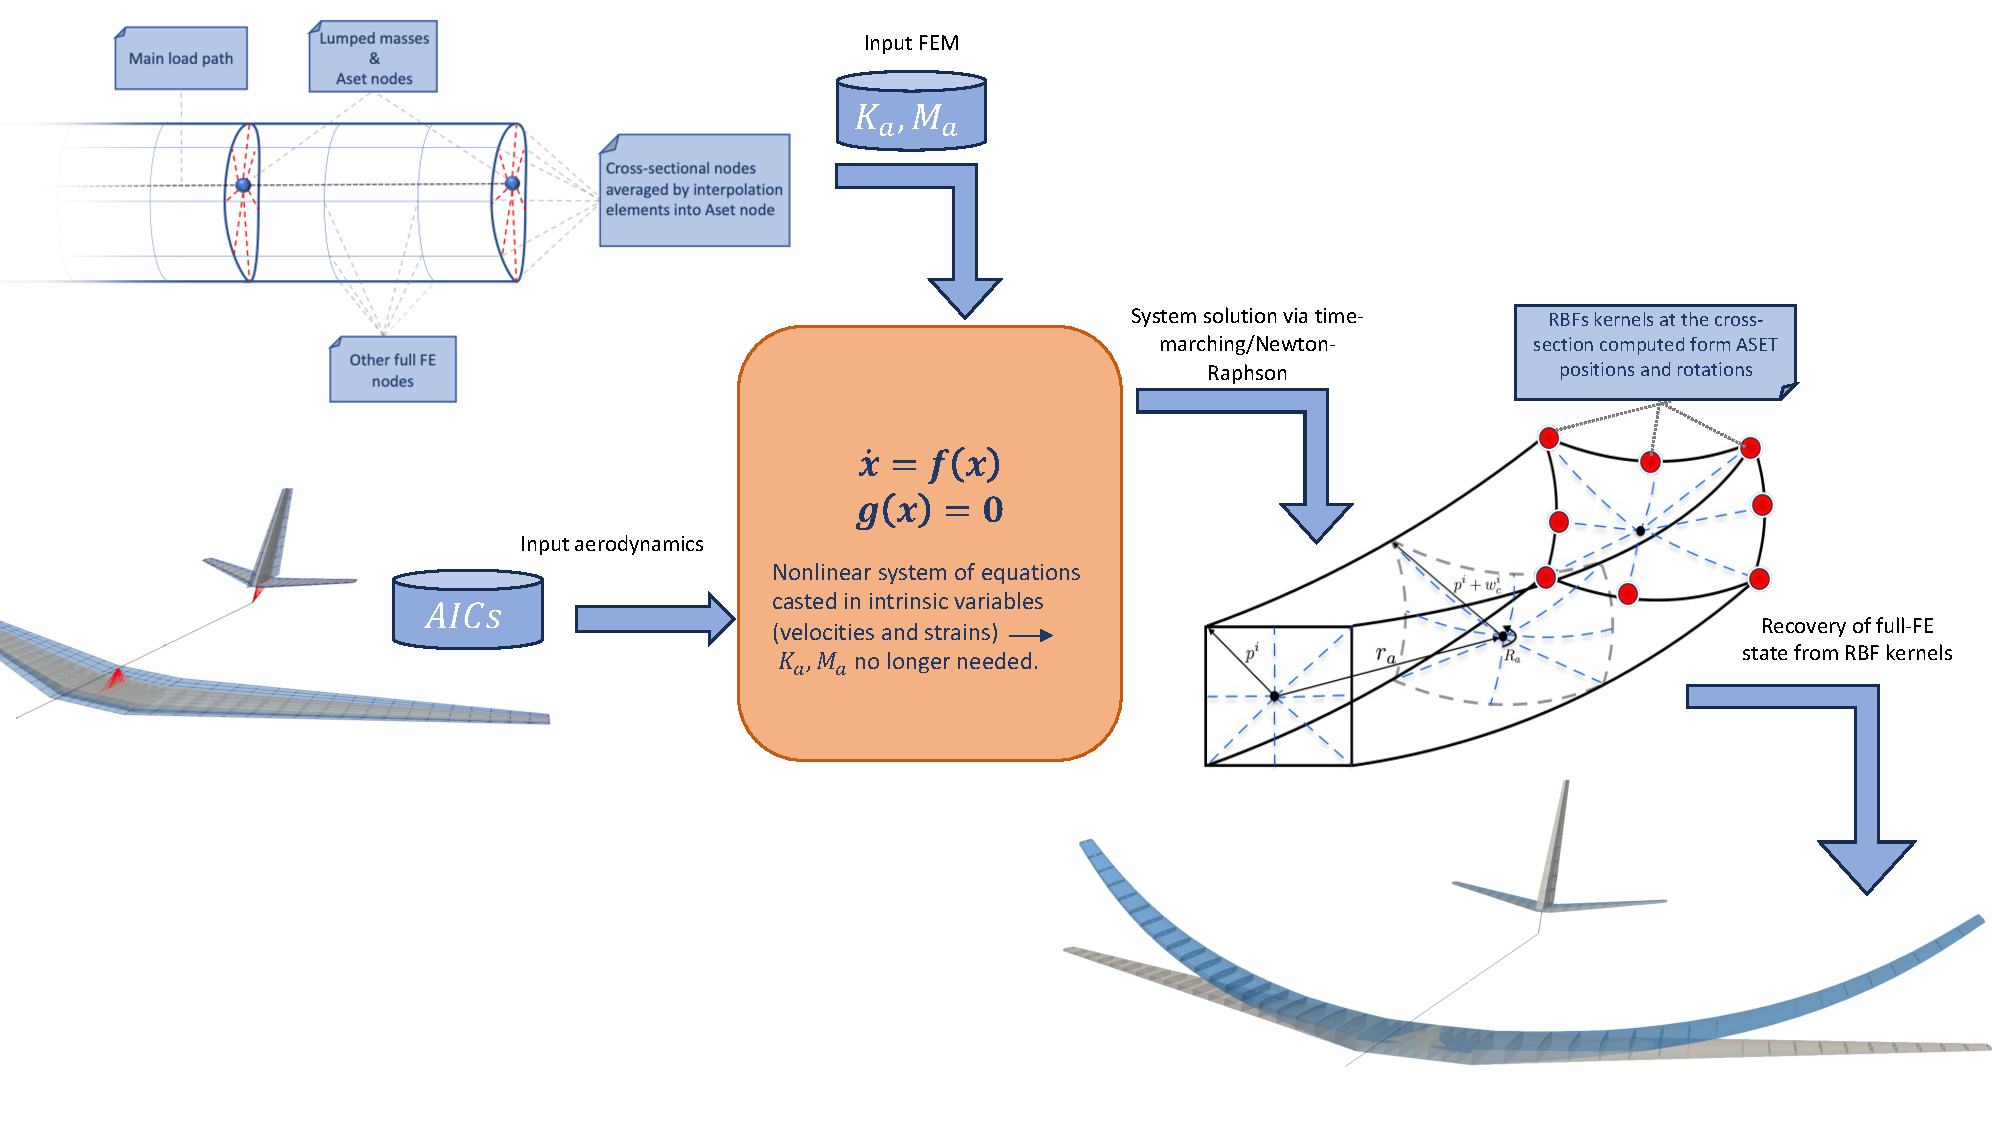
\includegraphics[width=1.\textwidth]{./figs/workflow2.pdf}
\caption{\label{fig:org4803a6a}Workflow of the solution process}
\end{figure}

This process of enhancing the linear 3D model with geometric nonlinearities along the slender dimension relies on the main assumption that cross-sectional deformations of the solid body in the reference configuration are not coupled to the this dimension as moving through configurations in time. As a result, distributed internal stresses act only through the normal of the cross-sections in the undeformed configuration \cite{CEA2021a}.
Applying the appropriate integration over the cross sectional reference area of the distributed traction forces, a Cosserat rod model is built, where the deformed state on the full domain is approximated by a deformable space curve \(\Gamma\) -- identified with the aircraft major load-paths. The primary variables  are the local inertial (linear and angular) velocities, grouped in the variable \(\bm{x}_1(s, t)\), and internal force and moments combined in \(\bm{x}_2(s, t)\). They are function of the 1D spatial dimension, \(s\), and time, \(t\). 
Applied forces and moments per unit length, \(\bm{f}_1\), come naturally as follower forces and moments respectively. The equations are well described in \cite[Ch. 8]{PALACIOS2023}.
Constitutive properties are given by the compliance matrix, \(\bm{\mathcal{C}}\), relating sectional forces and moments to strains and curvatures and the sectional mass matrix, \(\bm{\mathcal{M}}\), linking velocities and momenta. Finding a good approximation to these matrices is a common challenge in formulations that aim to build nonlinear 1D models from full FE models. This work circumvents having to calculate explicit expressions of \(\bm{\mathcal{C}}\) and \(\bm{\mathcal{M}}\) by solving the equations in modal space and linking them to the modal shapes and their derivatives as first described in \cite{PALACIOS2012}.

Using the intrinsic modes and the projection of the state variables, a Galerkin projection is carried out such that \(\pmb{x}_1 = \pmb{\phi}_1\pmb{q}_1\) and \(\pmb{x}_2 = \pmb{\phi}_2\pmb{q}_2\) and the equations of motion take the following form:

\begin{equation}
\label{eq2:sol_qs}
\begin{split}
\dot{\pmb{q}}_{1} &=  \pmb{\omega} \odot  \pmb{q}_{2} - \pmb{\Gamma}_{1} \pmb{:} \left(\pmb{q}_{1} \otimes \pmb{q}_{1} \right) - \pmb{\Gamma}_{2} \pmb{:} \left( \pmb{q}_{2} \otimes  \pmb{q}_{2} \right) + \bm{\eta}  \\
\dot{\pmb{q}}_{2} &= -\pmb{\omega} \odot \pmb{q}_{1} + \pmb{\Gamma}_{2}^{\top} \pmb{:} \left( \pmb{q}_{2} \otimes  \pmb{q}_{1} \right)
\end{split}
\end{equation}
where \(\odot\) is the  Hadamard product (element-wise multiplication), \(\otimes\) is the tensor product operation and \(\pmb{:}\) is the double dot product\footnote{The double dot product, commonly found in solid mechanics descriptions, represents a contraction of the last two indexes of the first tensor with the first two indexes of the second one; it however needs further specification as two alternative definitions can be adopted and here we opt for the following: \(\pmb{a} \pmb{:} \pmb{b} = a_{..ij} b_{ij..}\). This has implications on the definition of the transpose of \(\bm{\Gamma}_2\) in the second equation since for high order tensors multiple transpose operators can be defined. Consistency is achieved by ensuring the dot product operation satisfies the following: \(\pmb{x} \cdot \left(\bm{\Gamma} \pmb{:} \left( \pmb{y} \otimes \pmb{z} \right)  \right) = \pmb{y} \cdot \left(\bm{\Gamma}^{\top} \pmb{:} \left(\pmb{z} \otimes \pmb{x} \right)  \right)\), which leads to the transpose of the third order tensor, \(\bm{\Gamma} = \Gamma^{ijk}\), as \(\bm{\Gamma}^{\top} = \Gamma^{jki}\).}.
The new form of the equations in compact tensorial notation is in fact the way they have been implemented and vectorised. This description is geometrically-exact with quadratic nonlinearities only, encapsulated in the nonlinear modal couplings of the third-order tensors \(\pmb{\Gamma}_{1}\) and \(\pmb{\Gamma}_{2}\) (the former introduces the gyroscopic terms in the dynamics and the latter introduces the strain-force nonlinear relation). \(\pmb{\eta}\) is the modal projection of the external forcing terms. They are computed as integrals along the load-path 1D domain as an inner product: \(\langle \pmb{u},\pmb{v}  \rangle = \int_\Gamma \pmb{u}^\top \pmb{v} ds\), for any \(\pmb{u}\in\mathbb{R}^6\) and \(\pmb{v}\in\mathbb{R}^6\):
\begin{align}\label{eq2:gammas12}
\Gamma_{1}^{ijk} & = \langle \pmb{\phi}_{1i}, \lo_1(\pmb{\phi}_{1j})\pmb{\psi}_{1k}\rangle, \nonumber \\
\Gamma_{2}^{ijk} & = \langle \pmb{\phi}_{1i}, \lo_2(\pmb{\phi}_{2j})\pmb{\psi}_{2k}\rangle,  \\
\eta_{i} & = \langle \pmb{\phi}_{1i}, \pmb{f}_1\rangle  \nonumber
\end{align}
where \(\lo_1\) and \(\lo_2\) are linear operators, \(\pmb{\psi}_1 = \bm{\mathcal{M}}\pmb{\phi}_1\) and \(\pmb{\psi}_2 = \bm{\mathcal{C}}\pmb{\phi}_2\) are also cast as momentum and strain mode shapes and approximated using the Linear Normal Modes of the FE model. In other words, each natural vibration mode can be uniquely expressed in terms of velocity, force/moment, momentum, or strain variables. While those would be redundant in a conventional linear vibration analysis, they will enable to identify all the coefficients in Eqs. \eqref{eq2:sol_qs}.
\subsection{formulas}
\label{sec:orgc6aff4b}
$$
\bm \Gamma_1 = einsum('isn,jskn->ijk', \bm \phi_1, \mathcal{v}())
$$

\subsection{placeholder}
\label{sec:org6871729}

The corresponding distribution of linear and rotational momenta at the master nodes can be  obtained using the condensed inertia matrix, \(\pmb{\Psi}_{1j}  = \pmb{M}_a \pmb{\Phi}_{1j} = \pmb{M}_a \pmb{\Phi}_{0j}\), expressed in their components in the global frame of reference. The introduction of this momentum mode has allowed calculations to be performed on distributed mass models and the use of any type of condensation technique. Because the mass matrix is already calculated as an integral along the 3D domain and then condensed to a set of master nodes, the continuous momentum mode shapes, \(\pmb{\psi}_1\), are considered lumped and defined as,
\%
\begin{equation}
\pmb{\psi}_{1j}(s) =  \pmb{\Xi}_{0}(s_i) \pmb{\Psi}_{1j,i}\delta(s-s_i)
\end{equation}
where \(\delta\) is Dirac's delta function. Each displacement mode also generates a corresponding internal stress state. This defines discrete force/moment modes, \(\pmb{\Phi}_{2}\), which are obtained from the displacement modes and the condensed stiffness matrix using a summation-of-forces approach from aircraft load analysis, \cite[Ch. 18]{Wright2007}. If \(N_n\) is the total number of nodes, the internal node forces are for each mode \(j\) computed as \(\bm{\mathfrak{f}}_{(j)}  = \pmb{K}_a\pmb{\Phi}_{0j}^{1-3}\), with \(\bm{\mathfrak{f}}_{(j)} \in \mathbb{R}^{3N_n}\); and analogously the internal moments as \(\bm{\mathfrak{m}}_{\mathfrak{f}(j)}  = \pmb{K}_a\pmb{\Phi}_{0j}^{4-6}\). Next, a function \(\mathcal{S}(\bm{\mathfrak{h}},s_i)\) is defined so that it sums the  value of \(\bm{\mathfrak{h}}\) at each node in the path from a free end to the node \(s_i\) in the structure. \(\pmb{\Phi}_{2}\) is calculated as
\%
\begin{align}\label{eq:phi2}
\pmb{\Phi}_{2j,i+\frac{1}{2}}&= \begin{bmatrix}\mathcal{S}(\bm{\mathfrak{f}}_{(j)},s_i)\\  \mathcal{S} \left( \bm{\mathfrak{m}}_{\mathfrak{f}(j)} + (\bm{r}_i-\bm{r}_{i+\frac{1}{2}}) \times \bm{\mathfrak{f}}_{(j)},s_i \right)
\end{bmatrix} 
\end{align}
\%
where \(\pmb{r}_i\) is the position vector of the nodes summed by \(\mathcal{S}\), and \(\bm{r}_{i+\frac{1}{2}}\) the mid position between nodes \(s_i\) and \(s_{i+1}\). The first term is the sum of forces due to modal displacements and the second one the sum of moments due to modal rotations and the cross product of the  position vector and the previous calculated force. This equation represents an equilibrium of internal forces and moments -- between node \(i\) and \(i+1\). Results are presented in the mid-point \(i+\frac{1}{2}\) because more information cannot be extracted in terms of linear stresses from one node to the other. \%Note, however, \(i+\frac{1}{2}\) corresponds to the \$i\$th raw in the matrix \(\pmb{\Phi}_{2}\) and free-end points of the structure have a value of zero. 
The sum \(\mathcal{S}\) is taken as positive in the direction of increasing \(s\), and negative otherwise, so that the addition of internal forces and moments from all nodes in the model equals zero. An algorithm to calculate the optimal path for this sum was designed. The continuous force modes, \(\pmb{\phi}_{2}\), are now interpolated as piece-wise constant between nodes,
\begin{align}
\pmb{\phi}_{2j}(s) &= \pmb{\Xi}_{0}(s_i) \pmb{\Phi}_{2j,i+\frac{1}{2}} 
\end{align}
with \(s \in [s_i,s_{i+1}]\), as before. Finally, the strain modes \(\pmb{\psi}_{2}\) are obtained from spatial derivatives of the displacement modes along \(\Gamma\), following Eq. \eqref{eq2:linear CPhi2}, and interpolated as piece-wise constant too,
\begin{align}\label{eq2:psi2}
\pmb{\psi}_{2j}(s) = -\frac{\pmb{\phi}_{1j}(s_{i+1})-\pmb{\phi}_{1j}(s_{i})}{\Delta s_{i}}+ \pmb{E}^\top\frac{\pmb{\phi}_{1j}(s_{i+1})+\pmb{\phi}_{1j}(s_{i})}{2} 
\end{align}

\subsection{Nonlinear aeroelastic system}
\label{sec:org7092880}
The full aeroelastic solution is described extending Eq.  \eqref{eq2:sol_qs} with gravity forces, \(\bm{\eta}_g\), aerodynamic forces and gust disturbances, \(\bm{v}_g\). Control states can also be included \cite{CEA2021a}, but they are not necessary for this work. For a set of reduced frequencies and a given Mach number, the DLM (or a higher fidelity aerodynamic method) yields the Generalised Aerodynamic Forces (GAFs). The current implementation uses Roger's rational function approximation to those GAFs, which results in the follower modal forces:

\begin{equation}\label{eq3:eta_full}
\begin{split}
\bm{\eta}_a = \tfrac12\rho_\infty U_\infty^2 & \left(\vphantom{\sum_{p=1}^{N_p}} \pmb{\mathcal{A}}_0\bm{q}_0 +\frac{c}{2U_\infty}\pmb{\mathcal{A}}_1 \bm{q}_1 +\left(\frac{c}{2U_\infty}\right)^2 \pmb{\mathcal{A}}_2\dot{\bm{q}}_1   \right.  \\
& \left. + \pmb{\mathcal{A}}_{g0}\bm{v}_g +\frac{c}{2U_\infty}\pmb{\mathcal{A}}_{g1} \dot{\bm{v}}_g +\left(\frac{c}{2U_\infty}\right)^2 \pmb{\mathcal{A}}_{g2}\ddot{\bm{v}}_g +  \sum_{p=1}^{N_p} \pmb{\lambda}_p  \right) 
\end{split}
\end{equation}

The coupling of the structure and aerodynamic equations combined with the aerodynamic lags gives the final ODE system: 

\begin{equation}
\label{eq2:sol_qs}
\begin{split}
\dot{\pmb{q}}_{1} &=  \hat{\pmb{\Omega}}  \pmb{q}_{2} - \hat{\pmb{\Gamma}}_{1} \pmb{:} \left(\pmb{q}_{1} \otimes \pmb{q}_{1} \right) - \hat{\pmb{\Gamma}}_{2} \pmb{:} \left( \pmb{q}_{2} \otimes  \pmb{q}_{2} \right) + \hat{\bm{\eta}}  \\
\dot{\pmb{q}}_{2} &= -\pmb{\omega} \odot \pmb{q}_{1} + \pmb{\Gamma}_{2}^{\top} \pmb{:} \left( \pmb{q}_{2} \otimes  \pmb{q}_{1} \right) \\
\dot{\bm{\lambda}}_{p} &= \hat{\bm{\mathcal{A}}}_{p+2}\pmb{q}_{1}
                       + \hat{\bm{\mathcal{A}}}_{p+2}\dot{\pmb{v}}_g
                       -\frac{2U_\infty\gamma_p}{c}\bm{\lambda}_{p}
\end{split}
\end{equation}
in this system the aerodynamic added-mass effect has been moved to the left hand side such that \(\bm{\mathrm{A}}_2 = (\pmb{I} - \frac{\rho c^2}{8}\pmb{\mathcal{A}}_2)^{-1}\), and it couples all DoF in \(\pmb q_1\). Thus the natural frequency terms become \(\hat{\pmb{\Omega}} = \bm{\mathrm{A}}_2 diag(\pmb{\omega})\) and the nonlinear terms \(\hat{\pmb{\Gamma}} = \bm{\mathrm{A}}_2 \bm{\Gamma}\). The effect of all external forces, aero, \(\bm{\eta}_a\), gravity, \(\bm{\eta}_g\), and others, \(\bm{\eta}_f\), are combined in such that \(\hat{\bm{\eta}} = \bm{\mathrm{A}}_2 \left( \left( \bm{\eta}_a - \frac{\rho c^2}{8} \pmb{\mathcal{A}}_2\dot{\bm{q}}_1 \right) +  \bm{\eta}_g + \bm{\eta}_f \right)\). \\
Note that the structure of the formulation in modal space naturally leads to reduced order models and easily caters for vectorised operations. For instance, the contraction of \(\bm \Gamma_2^T{\top}\) in the second equation of Eqs. \ref{eq2:sol_qs} is implemented as an Einstein summation in JAX as \texttt{einsum(ijk,ki->j, gamma2, tensordot(q2, q1, axes=0)}. This will be briefly discussed next. 
\subsection{Computational implementation}
\label{sec:org7909629}
The main contribution of this work is a new computational implementation that achieves accelerations of over 2 orders of magnitude with respect to its predecessor\footnote{:Both the new implementation and the examples of this paper can be found at \url{https://github.com/ImperialCollegeLondon/FEM4INAS}.}. In addition, a highly modular, flexible architecture based on software design patterns has been put in place, which was further described in \cite{CEA2024}. Moreover, the resulting nonlinear aeroelastic framework is suitable for modern hardware architectures and the computation of sensitivities via algorithmic differentiation (AD) has been implemented as a crucial part for design optimisation, both of which will be exemplified in future work.

The key enabler was moving from standard Python to a highly vectorised, JAX-based numerical implementation. JAX is a Python library designed for high-performance numerical computing with focus on machine learning activities \cite{jax2018github}. This library is developed and maintained by Google research team. It combines XLA (accelerated linear algebra) and Autograd, the former being a compiler that optimises models for different hardware platforms, the latter is an Automatic Differentiation (AD) tool in Python. 
Moreover, its extensible system of composable function transformations provides a set of important features for Computational Science as illustrated in Fig. \ref{fig:JAX-overview}. For instance, the vmap function allows for complex \textbf{vectorisation} operations and the pmap function for Single-Program Multiple-Data (SPMD) \textbf{parallelisation}. Both forward and reverse mode \textbf{automatic differentiation} are supported. Finally the \textbf{just-in-time compilation} (jit) relies on the XLA engine to compile and execute functions on CPUs but also on accelerators such as GPUs and TPUs, offering a versatile solution for seamlessly connecting the software to various types of hardware without requiring extra CUDA code, or a Domain Specific Language (DSL).

\begin{figure}[htbp]
\centering
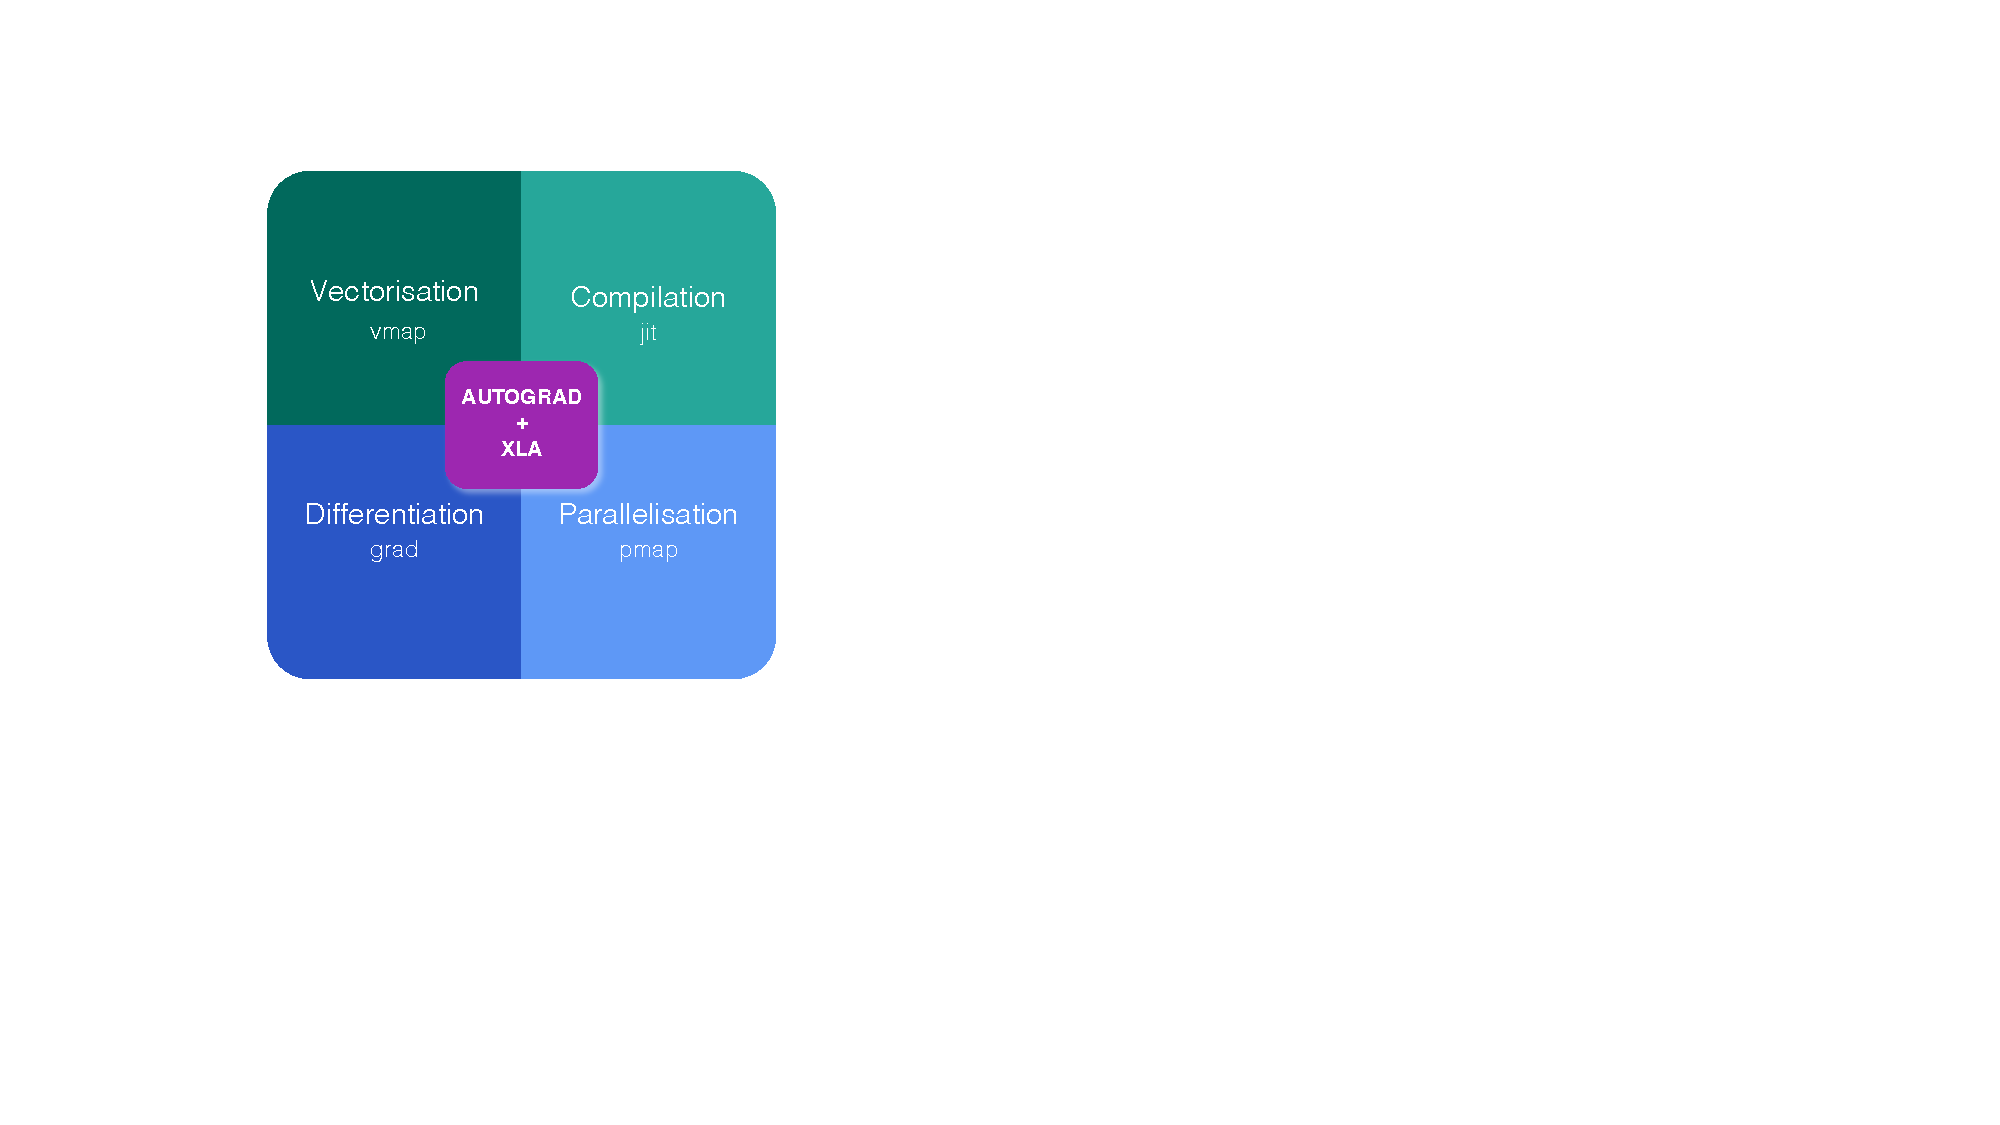
\includegraphics[width=0.35\textwidth]{./figs/jaxlogo2.pdf}
\caption{\label{fig:JAX-overview} JAX capabilities for modern scientific computing}
\end{figure}
The new capabilities come at the expense of a higher restriction in the way the code is written. Compilation and transformations in JAX only work for functionally pure programs, which pushes the software to comply with a nonconventional functional paradigm. Some of these characteristics are \textbf{pure functions}, i.e. functions that have no side effects, \textbf{input/output} stream management needs to be placed outside the numerical algorithms, \textbf{inmutability} of arrays, and \textbf{function composition}, or the ability to create functions by chaining other callables.

These very constraints allow to achieve the capabilities describe above via the many abstractions implemented internally in the library.

\section{Examples}
\label{sec:org8e113e6}
The cases presented are a demonstration of our solution approach to manage geometric nonlinearities, the accuracy of the solvers when compared to full FE simulations, and the computational gains that can be achieved.
All computations are carried out on a single core of the same CPU, an i7-6700 with 3.4 GHz clock speed.
\section{Conclusions}
\label{sec:org43c9622}
\bibliographystyle{plain}

\bibliography{../../../../../Documents/Engineering}
\end{document}
